\documentclass[a4paper,10pt]{article}

\usepackage[utf8]{inputenc}
%\usepackage[T1]{fontenc}

\usepackage{textcomp}           % Extra Symbole (Grad Celsius etc.)
\usepackage{amssymb,amsmath}    % Schöne Formeln (AMS = American Mathematical Society)
\usepackage{graphicx}           % Bilder und Seitenränder
\usepackage{subcaption}			% captions for subfigures
\usepackage{booktabs}           % Schönere Tabellen
\usepackage{colortbl}           % Farbige Tabellen
\usepackage{gensymb}
%\usepackage{tcolorbox}			% schöne bunte Boxen
\usepackage{mathtools}			% \mathclap für ordentliche \underbrace-			environments
\usepackage[left=2cm,right=2cm,top=2cm,bottom=2cm]{geometry}			% Pagelayout mit \newgeometry, \restoregeometry
\usepackage{float}
\usepackage{wrapfig}
\usepackage{enumitem}
\usepackage{float}
\usepackage{braket}
\usepackage{caption}
\usepackage{verbatim}
\usepackage[per-mode=reciprocal,output-decimal-marker={.},binary-units=true,separate-uncertainty=true]{siunitx}
\usepackage[breaklinks=true,colorlinks=true,linkcolor=blue,urlcolor=blue,citecolor=blue]{hyperref}
\usepackage{physics}
\usepackage{url}
\usepackage{subcaption}
\usepackage{calrsfs}
\usepackage{tikz}
\usetikzlibrary{decorations, positioning, intersections, calc, shapes,arrows, scopes}
\DeclareMathAlphabet{\pazocal}{OMS}{zplm}{m}{n}

\graphicspath{{./img/}}

\newcommand{\dif}{\mathrm{d}}

\bibliographystyle{instant}

\renewcommand{\k}{\mathbf{k}}
\begin{document}
\begin{titlepage}
 \begin{center}
 \Large{Lab Course in Experimental Physics: Optics}
 \end{center}
 \begin{center}
  \LARGE{\textbf{Focus locking of a tunable lens for optical transportation of ultracold atoms}}
 \end{center}
 \begin{center}
 \large Marco \textsc{Canteri} \\
 marco.canteri@student.uibk.ac.at\\
 \end{center}

 \begin{center}
 \vspace{1cm}
 Innsbruck, \today
 \vspace{1cm}
 \end{center}

 \begin{abstract}
In this project a setup for optical transportation of ultracold atoms has been realized. The focus of a laser was shifted with a tunable optotune lens controlled by custom electronics, and locked with a feedback signal generated from a quadrant photodiode.
\end{abstract}
  \vspace{1cm}

 \begin{center}
 
\includegraphics[scale=0.567]{img/uibk}
 \end{center}

\end{titlepage}

\section{Introduction}
Transportation of atoms has became an important technique for manipulating and studying quantum gases and ultracold atoms. Moving the atoms allows to prepare the atomic cloud in a chamber and studying such clound in another region equipped with the appropriate instruments. Several approaches have been developed, such as magnetic transport or mechanically transporting the setup. In this experiment optical transportation is used, the idea is simple: atoms are loaded from the trap in a optical lattice which is then moved with a tunable lens. The crucial part of the experiment is to control the focus reliably, thermic drifts can move the focus resulting in losing control on the trapped atoms. Therefore, focus locking is needed. In this experiment a feedback loop is exploited to correct such drifts, the error signal is generated with a quadrant photodiode (QPD), it is then compared with a reference used to set the focus position and then fed back into the tunable lens.

\section{Theoretical background}
\subsection{Focus tunable lens}
The key element of this experiment is a focus tunable lens. Usually lenses are made of a transparent solid material and they are static. A tunable lens instead can be electronically reshaped to change the focus. Inside the lens there is a liquid sealed in a elastic polymer membrane. This membrane can be reshaped with an actuator that act on the membrane, by changing the current of the actuator the membrane is pressed and therefore it is possible to control the focus. An important note it is that due to the mechanically working principle, gravity can affect the performance of the lens and it is suggested to use it horizontally.
\begin{figure}[H]
\centering
\includegraphics[width = .7\textwidth]{tunablelens}
\caption{A focus tunable lens, the coil exerts pressure on the memebrane containing th eliquid cha its shape. Image from \cite{lens_datasheet}}
\end{figure}
\section{Experiment setup}
\begin{figure}[htp!]
    \centering
    \tikzstyle{block} = [draw, fill=blue!20, rectangle,
    minimum height=3em, minimum width=6em]
    \tikzstyle{sum} = [draw, fill=blue!20, circle, node distance=1cm]
    \tikzstyle{input} = [coordinate]
    \tikzstyle{output} = [coordinate]
    \tikzstyle{pinstyle} = [pin edge={to-,thin,black}]

\begin{tikzpicture}[auto, node distance=2cm,>=latex']
    \node [input, name=input] {};
    \node [sum, right of=input] (sum) {};
    \node [block, right of=sum,
            node distance=3cm] (system) {Optical setup};
    \node [sum, right of=system, node distance=3cm, pin={[pinstyle]above:$R$}] (output) {};
    \node [block, below of=system] (controller) {PID Controller};

  %  \draw [->] (sum) -- (system);
    \draw [->] (system) --  node {$X$}(output);
    \draw [->] (output) |- node[pos=0.01] {$-$} node {$R - X$} (controller);
    \draw [-] (controller) -|
        node [near end] {$Y$} (sum)-- (system);
\end{tikzpicture}
\caption{Sketch of the control loop. The output of the system $X$ is compared to the reference $R$. The difference is fed into the controller, and the output of the controller $Y$ is fed back into the system. }
\label{fig:control_loop}
\end{figure}
The setup prepared can be divided in two parts, the optical setup and the electronics part used to control the optics. The main idea of the experiment is to control and lock the focus of a 1064nm laser. This is done with an optotune EL-16-40-TC focus tunable lens \cite{lens_datasheet}. To lock the focus, a part of the beam has been send through a cylindrical lens, and then measured with a quadrant photodiode. The cylindrical lens deforms the spherical symmetry of the beam such that when projected on the photodiode, the light will not hit all the four quadrants uniformly. The signal generated from the quadrants can be used as a measure of relative focus, therefore we can feedback this signal to the lens and get focus locking. A sketch of the loop can be found in figure \ref{fig:control_loop}. $X$ is the value determined from the QPD as
\begin{equation}\label{eq:voltage}
X = \frac{V_A + V_D - (V_B+V_C)}{V_A+V_B+V_C+V_D}.
\end{equation}
$V_A,V_B,V_C,V_D$ refer to the voltage output of the four quadrants as showed in figure \ref{img:opticsetup}, so $V_A$ and $V_D$ are opposite quadrant, and the same for $V_B$ and $V_C$. The idea of this formula is that when the ellipse is centered, a different orientation and different axis ratio will produce a different value for $X$. This value can be both negative or positive depending on the ellipse's orientation, in fact if the ellipse is tilted such that it mainly hits the quadrant $A$ and $D$, the sum $V_A+ V_D$ is greater then $V_B+V_C$ and $X$ will be positive, viceversa for the ellipse rotated of $90^\circ$. These situations are showed in figure \ref{fig:ellipses}. $X$ is also normalized such that it does not depend on the laser power. The value $R$ can be set from the computer of from an internal reference in the circuit, it is used to move the focus. Since the lens is current drive, the output of the PID $Y$ must be converted from voltage to current before feeding back to the lens. In the next two sections the details of the optical setup and the electronics are presented.
\begin{figure}[H]
  \centering{}
  \begin{subfigure}[t]{0.3 \textwidth}
    \centering
    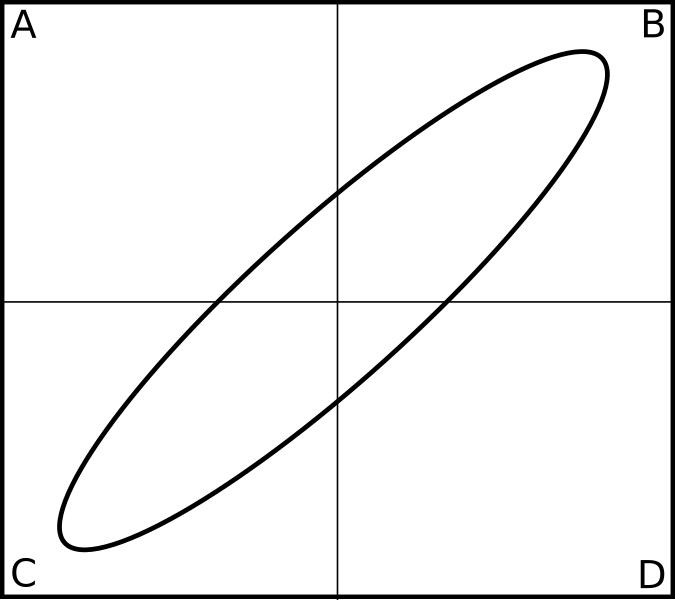
\includegraphics[width = \textwidth]{ellipse1}
    \caption{The ellipse is hitting manly $B$ and $C$, this will generate a negative signal}
  \end{subfigure}
  ~
  \begin{subfigure}[t]{0.3\textwidth}
    \centering
    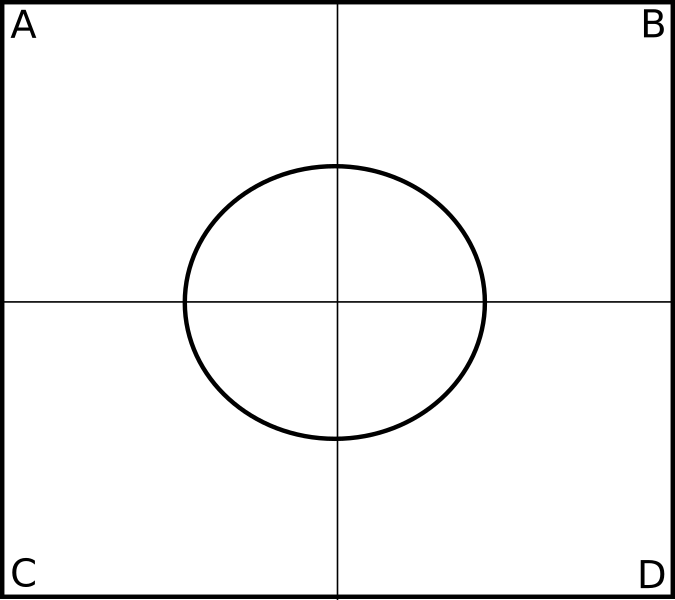
\includegraphics[width = \textwidth]{ellipse3}
    \caption{The ellipse is symmetric, thus the generated signal is 0}
  \end{subfigure}
  ~
  \begin{subfigure}[t]{0.3\textwidth}
    \centering
    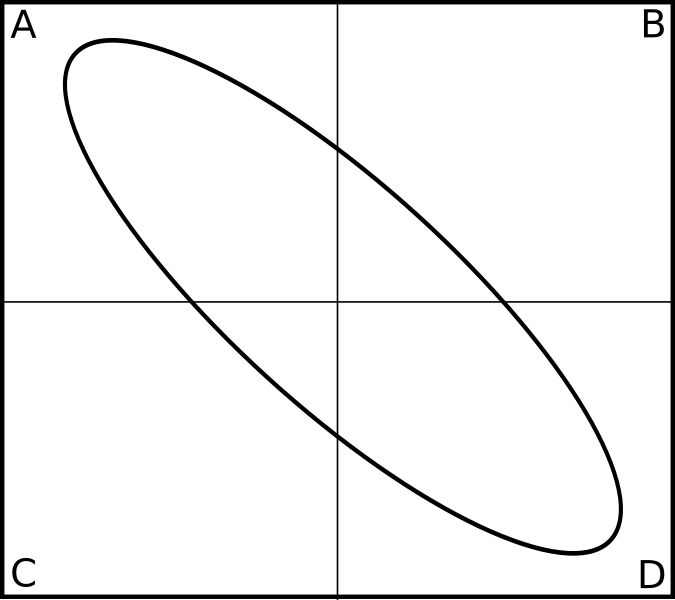
\includegraphics[width = \textwidth]{ellipse2}
    \caption{The ellipse is hitting manly $A$ and $D$, this will generate a positive signal}
  \end{subfigure}
  \caption{Extreme cases of ellipse projected on the quadrant photodiode.}
  \label{fig:ellipses}
\end{figure}
\subsection{Optical setup}
The setup is depicted in figure \ref{img:opticsetup}. We used a 1064nm laser, the light is split with a beam splitter, one beam is used in another experiment, while the beam showed in the setup is coupled with a fiber in order to filter the modes and have at the end a pure Gaussian beam. After the fiber the beam is expanded with two lenses to roughly 10 mm diameter. Subsequently, the beam pass through a tunable lens controlled by the electronic part. The lens can change focus from  -500 to +333 mm, but in this experiment we kept the focus negative. A beam splitter is used to create a beam for measuring the focus shift, while the transmitted beam is focused with a 400mm lens between point A and B depending on the current applied to the lens. The trick of using a tunable and a convergent lens instead of simply the optotune lens is to keep the waist of the beam constant, in fact a non constant beam would change trapping frequency and trap depth resulting in losing atom during the transportation \cite{opticaltransportation}.  Before the quadrant photodiode, the beam is reshaped by two cylindrical lenses of 100mm and 300mm focus length. One cylindrical lens would have been enough, but with two of them a better control over the shape can be achieved. This allows for a tuning of the QPD output, changing the shape will change the voltage output and therefore by moving the cylindrical lenses and the QPD, the working range of the QPD can be changed to better suit the specification of the electronic part.
\begin{figure}[H]
\centering
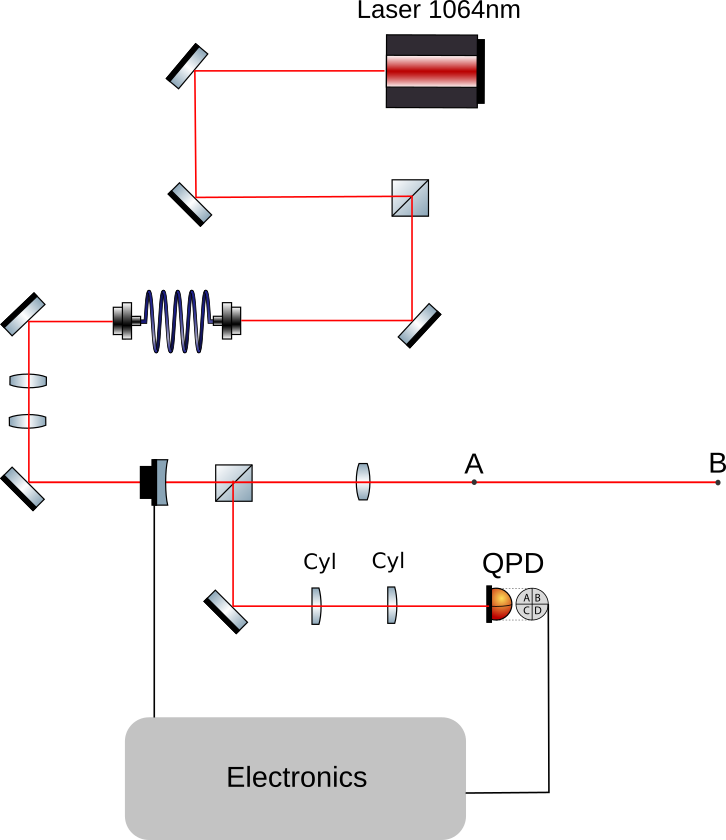
\includegraphics[width = .5\textwidth]{opticsetup}
\caption{Optical setup, after the fiber a 1064nm laser light is collimated and sent trough a tunable lens. Two cylindrical lens and a quadrant photodiode are used to generate an error signal for the focus which is feedback to the lens with some electronics. The focus of the laser could be changed from point A to point B, roughly 40 cm.} \label{img:opticsetup}
\end{figure}
\subsection{Electronic PID}
The electronics take care of driving the lens and calculating the feedback signal to lock the focus. The full circuit is in figure \ref{img:circuipid} and \ref{img:currentdriver}. The whole circuit was powered with $\pm18$ V from a power supply. This voltage has to be converted to $\pm 15$ V to power the QPD and the rest of the chips. This conversion has been done with the lower schematic shown is figure \ref{img:currentdriver}. Some filters has been included and four voltage regulators has been used to down convert the voltage.\\
In figure \ref{img:circuipid} out\_a,  out\_b, out\_c, out\_d are the four signals of the four quadrants. These has been summed with a operational amplifier OP470, and substracted with an INA111 to calculate all the needed quantities of equation \eqref{eq:voltage}. The division is performed by the chip AD734 using the configuration suggested by the datasheet in the section "DIVISION BY DIRECT DENOMINATOR CONTROL" \cite{ad734}. The output of the chip is $W = Y1\frac{X1}{U1}$, with these quantities referring to the pins of the chip. On the pin $Y1$ a trimmer is placed in order to have control on the gain of the chip. After the division, the result is compared with either an external reference or with an internal reference. Then, then substraction passes through the CMOS switch ADG441 such that the output can be grounded to shut down the PID part. Before the PID itself the signal travel through a stage of inverters in order to have the possibility to choose the sign of the signal. Finally we have the PID which lacks of the differential part, but we thought it was not necessary. The output if the final signal we want to send to the lens, but since the lens is current controlled, it must be converted. We take care of this in the schematic shown in figure \ref{img:currentdriver}. Here we can see another feedback loop with a PID. This is done to have a more stable current. The idea of converting a voltage to a current is to use a resistor and exploit Ohm's law, however attaching a load to the resistor would change the current flowing. Therefore we used a four wires resistor, the extra two pins are used to read the voltage on the resistor, compare it to our voltage signal and feed it back to the resistor. This is why a PID loop is used. Furthermore, since the lens requires high current (-250mA to 250 mA) two buffers are used to provide the necessary power.\\
A photo of the final circuit with the layout highlighted can be found in figure \ref{img:layout}.
\begin{figure}
\centering
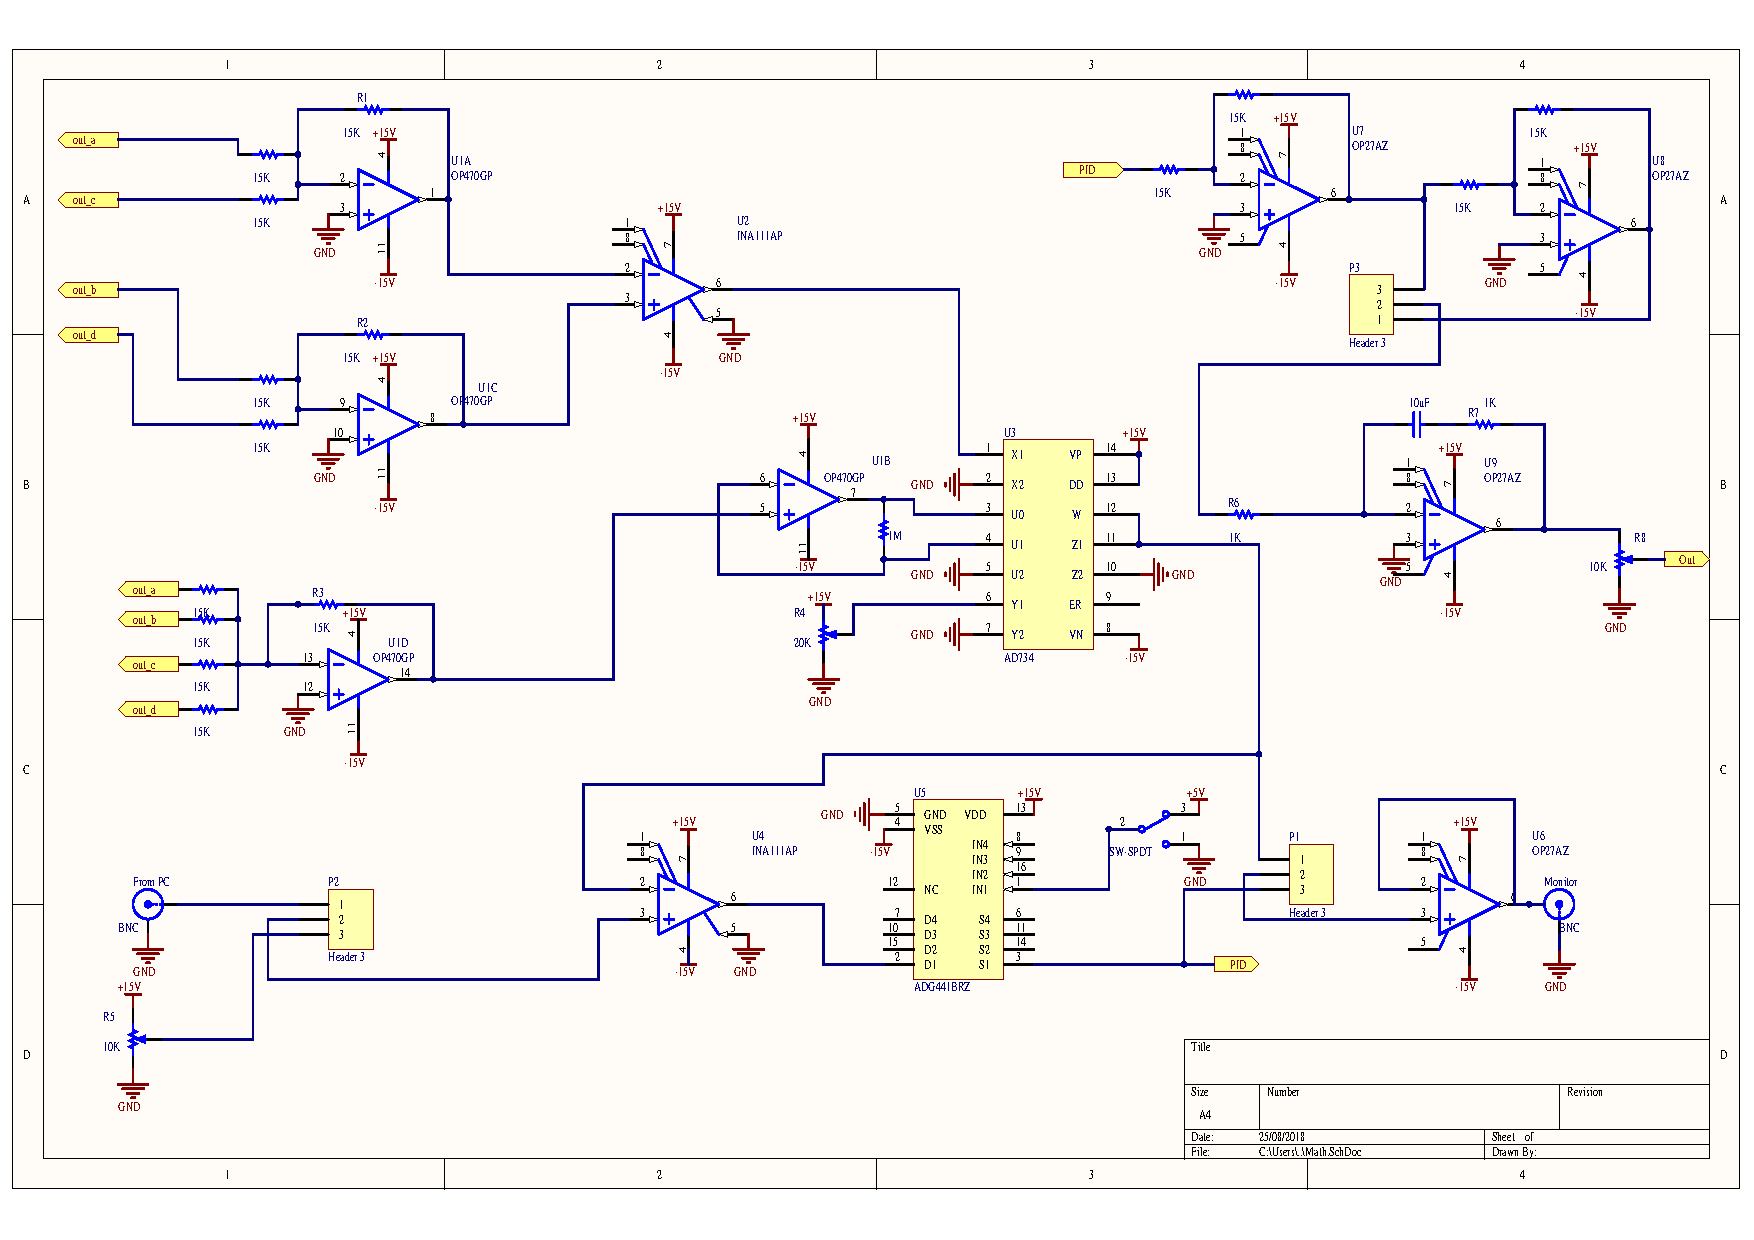
\includegraphics[width = \textwidth]{circuit/pid}
\caption{Schematic of the circuit. Full resolution image and original Altium file can be found here: \url{https://github.com/kante95/summer_lab/tree/master/circuit}} \label{img:circuipid}
\end{figure}
\begin{figure}
\centering
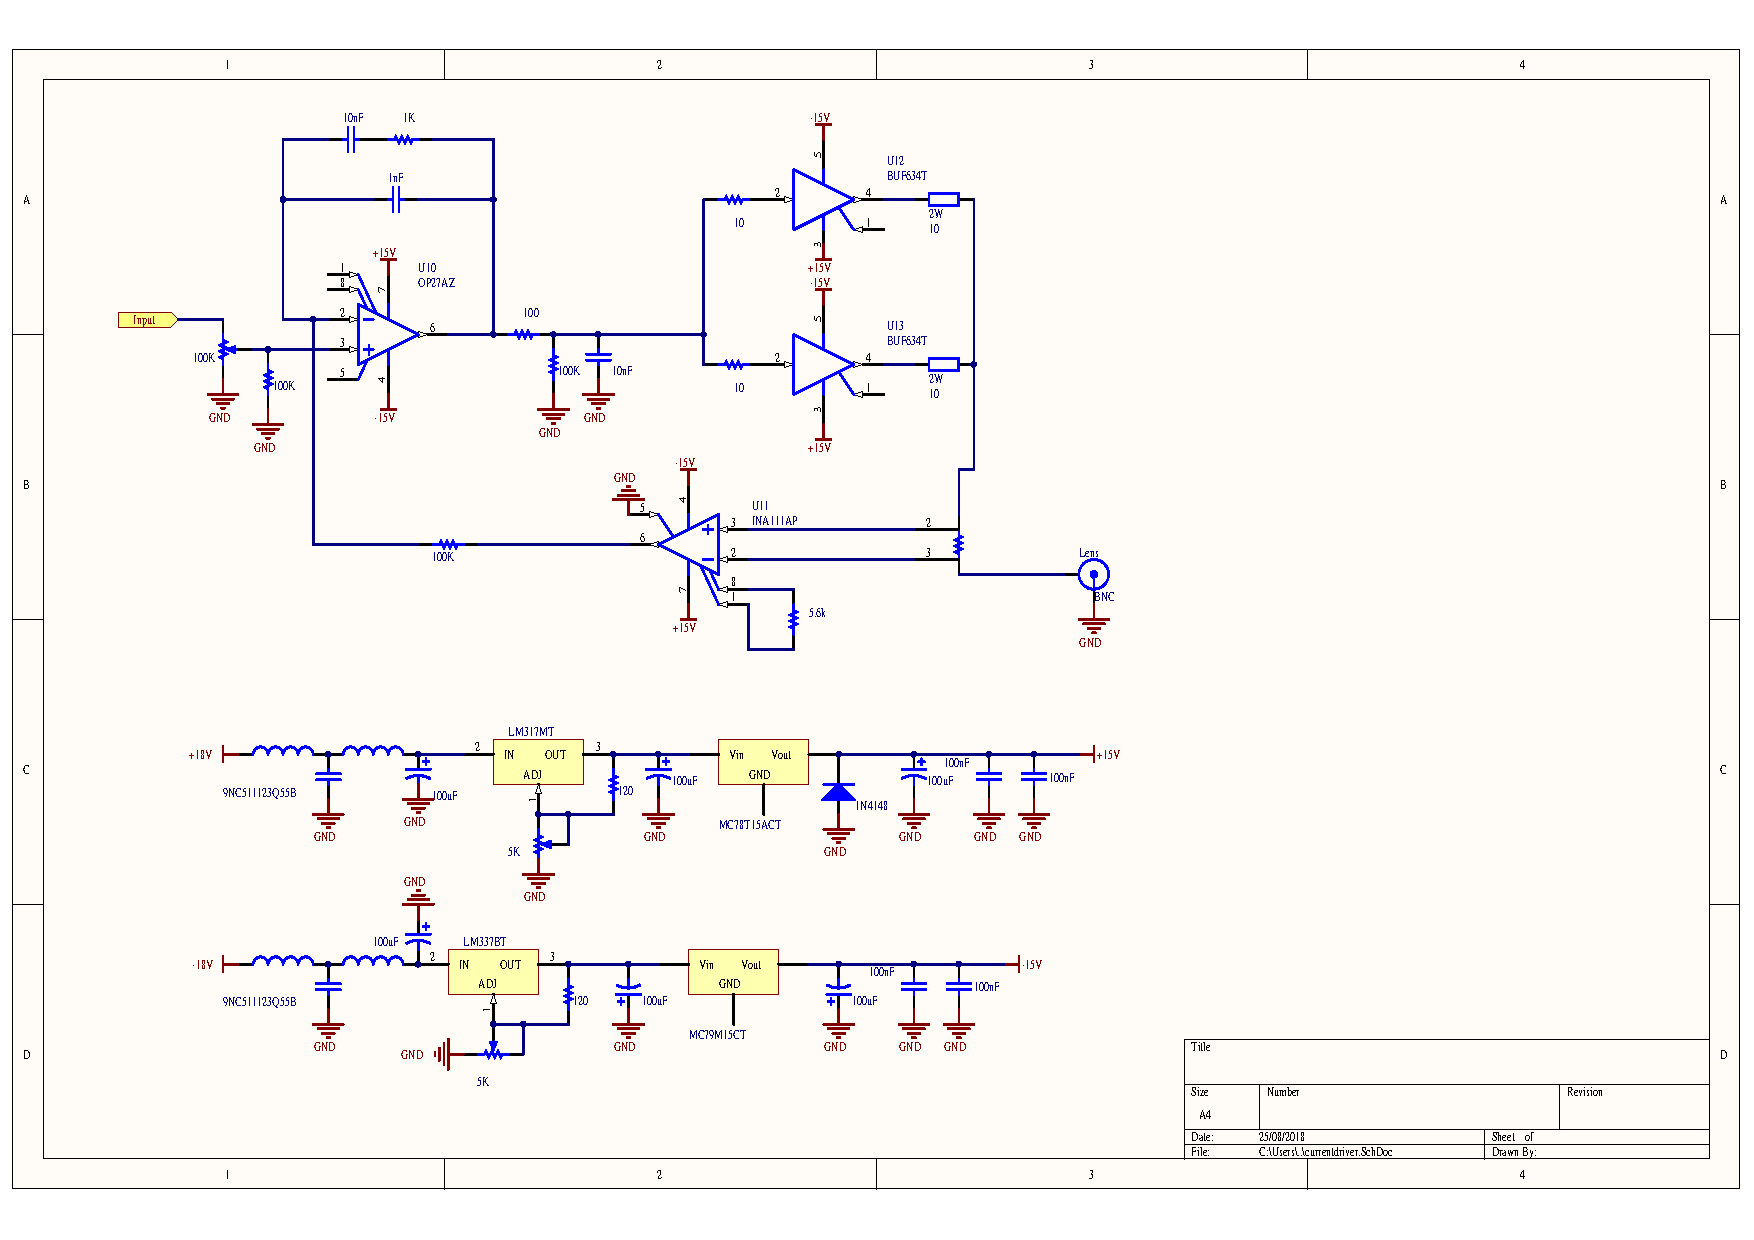
\includegraphics[width = \textwidth]{circuit/currentdriver}
\caption{Schematic of the circuit. Full resolution image and original Altium file can be found here: \url{https://github.com/kante95/summer_lab/tree/master/circuit}} \label{img:currentdriver}
\end{figure}
\begin{figure}
\centering
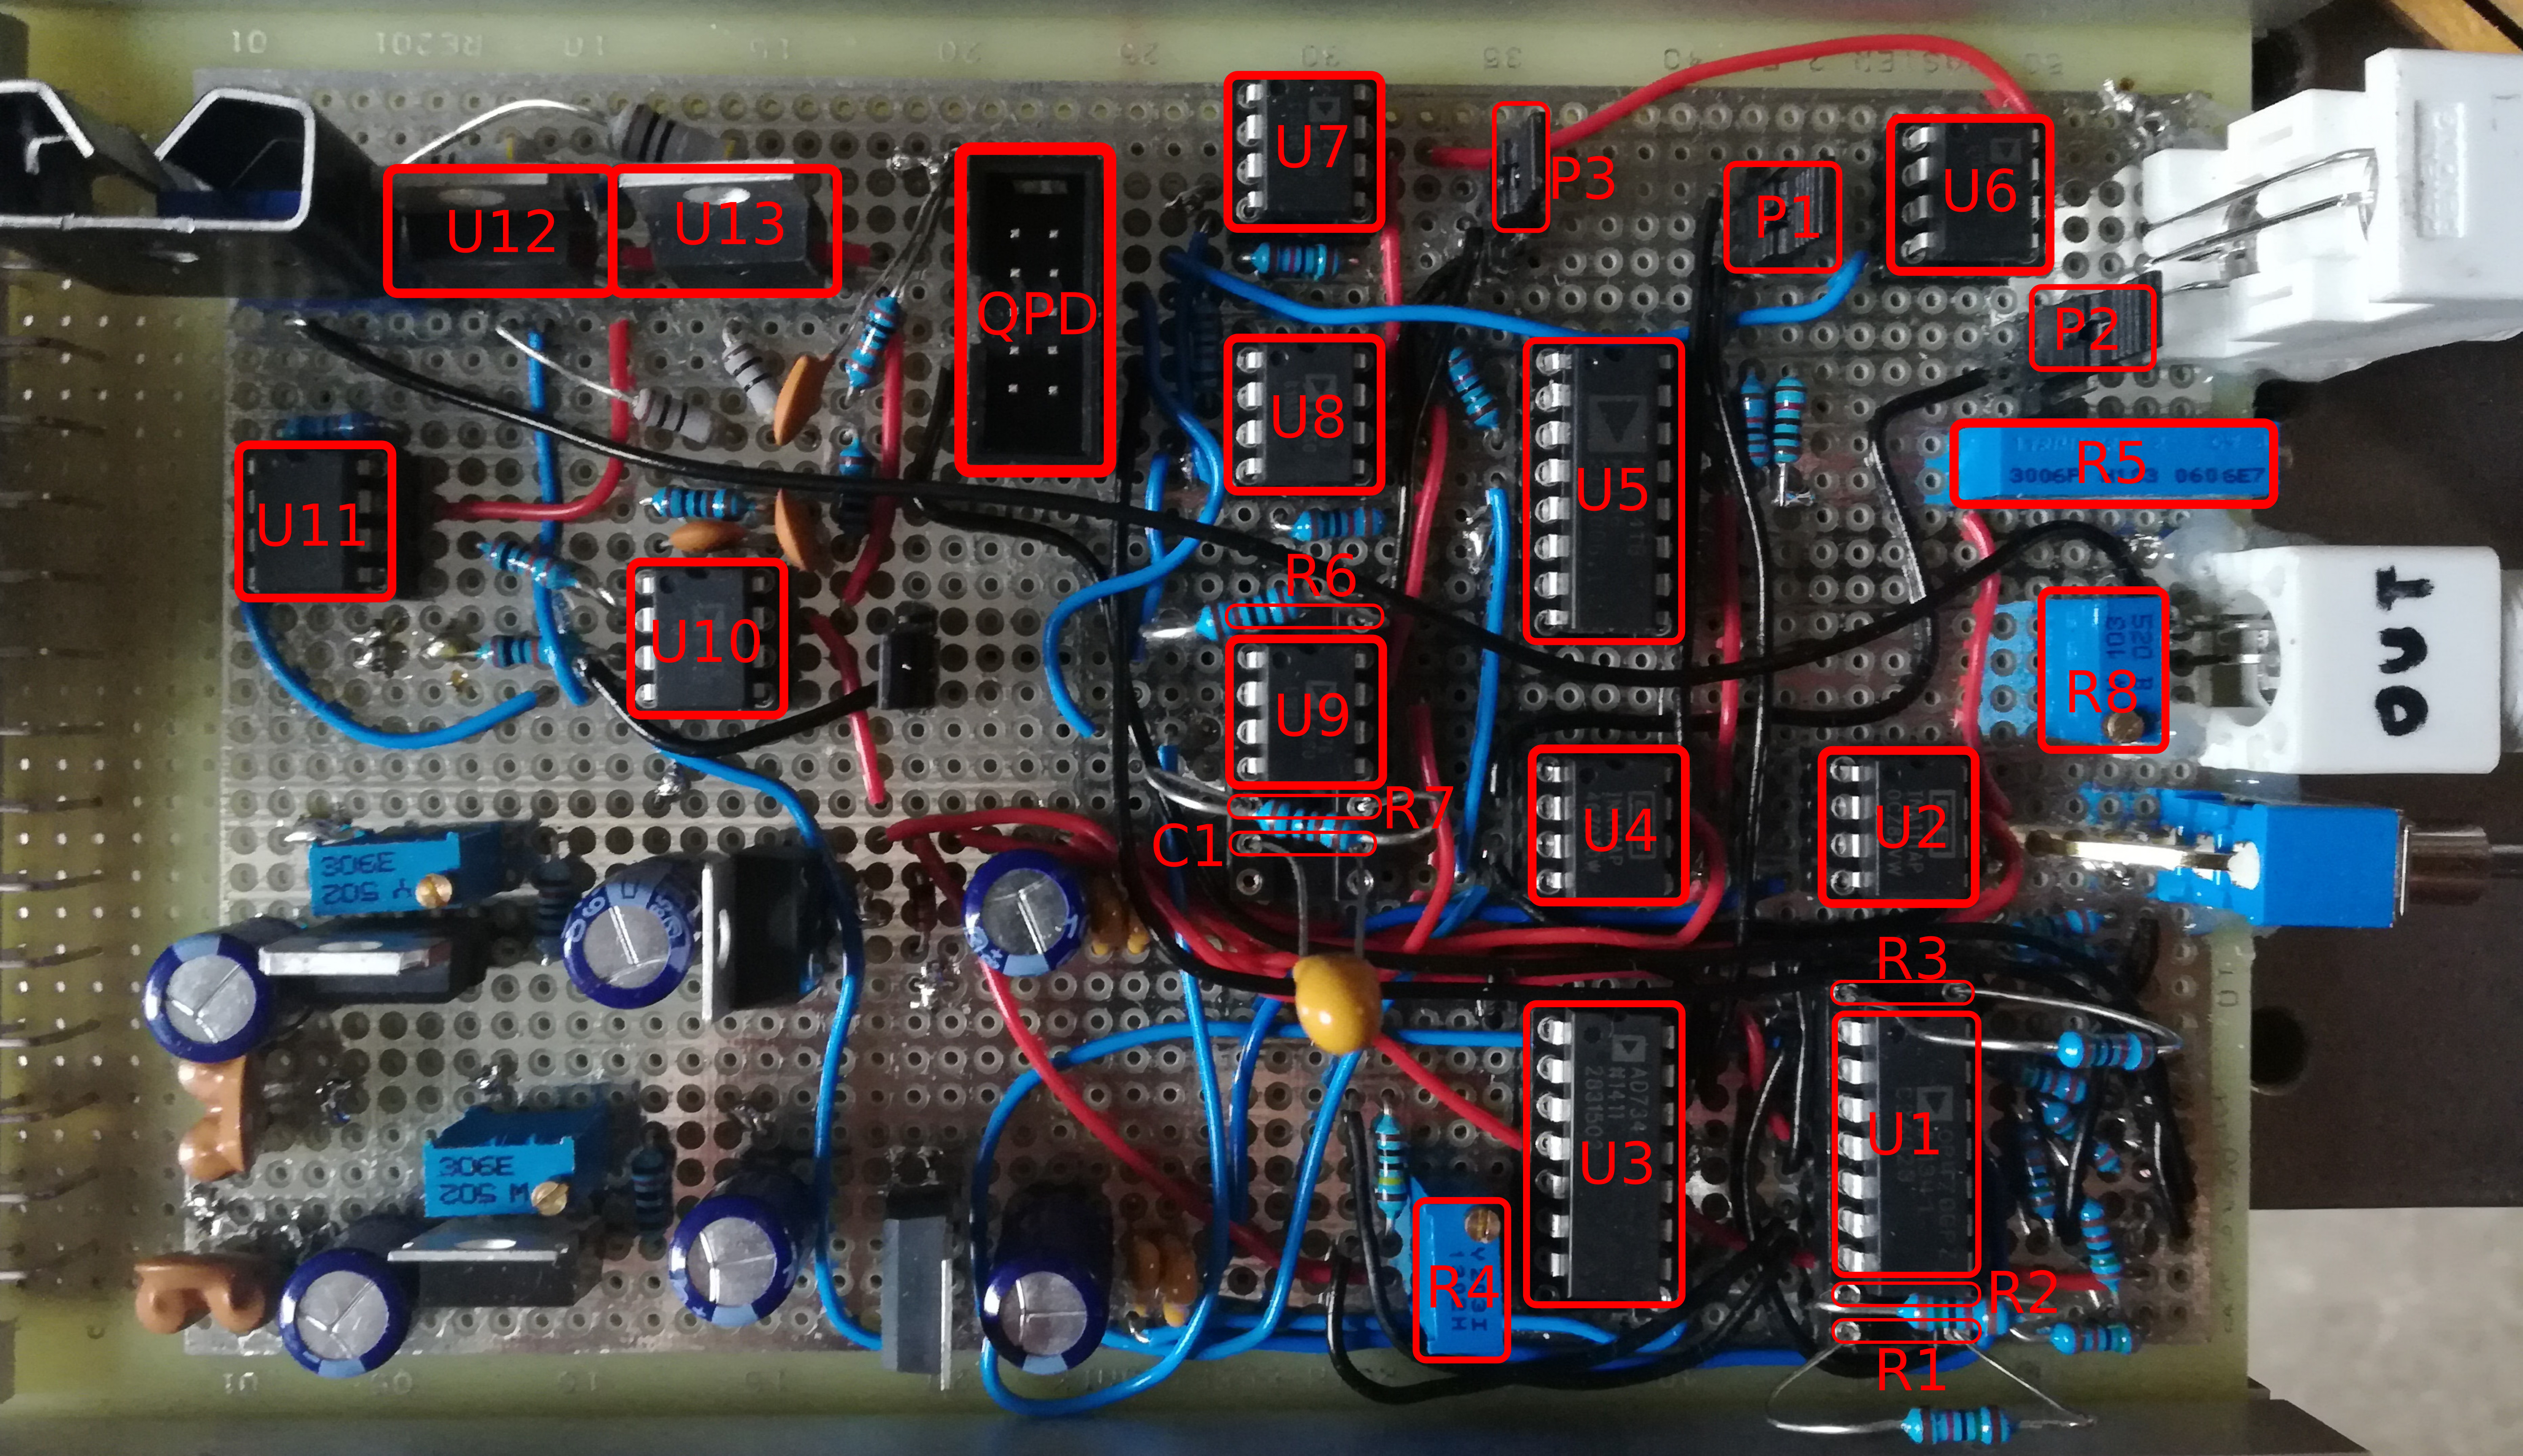
\includegraphics[width = \textwidth]{circuit/layout}
\caption{Real circuit. The parts numbers highlighted are shown in the schematic \ref{img:circuipid} and \ref{img:currentdriver}. Full resolution image can be found here: \url{https://github.com/kante95/summer_lab/tree/master/circuit}} \label{img:layout}
\end{figure}
\section{Conclusion}

 \begin{thebibliography}{99}
\bibitem{lens_datasheet}
 \textsc{Optotune}, \textit{EL-16-40-TC}, \url{https://www.optotune.com/images/products/Optotune%20EL-16-40-TC.pdf}
%
 \bibitem{opticaltransportation}
 \textsc{J. Léonard, M Lee, A. Morales, T. Karg, T Esslinger, T. Donner}, \textit{Optical transport and manipulation of an ultracold atomic cloud using focus-tunable lenses}, New Journal of Physics, volume 16 number 9, 2014
\bibitem{ad734}
\textsc{AD734 Datasheet}, \url{http://www.analog.com/media/en/technical-documentation/data-sheets/AD734.pdf}
%
% \bibitem{bergmann}
% \textsc{Bergmann-Schäfer}, \textit{Gase, Nanosysteme, Flüssigkeiten}, \textit{Band 5} (de Gruyter, 2005)
%
% \bibitem{cold_cathode}
% \textsc{LDS Vacuum Shopper}, \textit{Cold Cathode Gauges}, \url{http://www.ldsvacuumshopper.com/cocaga.html}
%
% \bibitem{script}
% \textsc{Jennifer Meyer, Roland Wester}, \textit{Versuch im Fortgeschrittenen Praktikum FP3: Supersonische Düsenstrahlen}
%
% \bibitem{lifetime}
% \textsc{Cullen P.J., Milosavljevic V.} (2015) Prog. Theor. Exp. Phys.2015/6, 063J01 . doi:10.1093/ptep/ptv070
%
% \bibitem{illinois}
% \textsc{McCall research group}, \textit{Supersonic Expansion Discharge Source}, \url{http://bjm.scs.illinois.edu/past/source.php}
 \end{thebibliography}
\end{document}
